\chapter[The Waterfall Target]{The Waterfall Target
\footnote{
  $CVS~revision~ $Id: waterfall-target.tex,v 1.2 2003/11/18 07:46:27 gen Exp $ $
}
\footnote{Authors: David Meekins \url{mailto:meekins@jlab.org} and 
 Maurizio Lucentini \url{mailto:lucentin@jlab.org}}
}
% \newcommand{\boldsymbol}[1]{\mbox{\boldmath $#1$}}

\section{Overview}

The Hall A Waterfall Target was developed by INFN Roma and will be
used by several aproved experiments in Hall A. The target may be configured
for one or multiple waterfall {}``foils''. Operation of the target
may be achived manualy (for experts only) or remotely using the Waterfall
Target GUI accessable from the standard Hall A controls screen. The
software is maintained by David Wetherholt of the accelerator controls
group. User operation of the target is achieved through this GUI only.
Any problems with the target must be addressed by and expert. A list
of experts is give in Table \ref{tab: experts}.%
\begin{table}
\begin{center}\begin{tabular}{|c|c|c|}
\hline 
Name &
Phone&
Pager\\
\hline
\hline 
Maurizio Lucentini&
-&
-\\
\hline
Dave Meekins&
5434&
872-2442\\
\hline
Ed Folts&
7857&
989-4580\\
\hline
Rusty Salmons&
6914&
820-9205\\
\hline
Scot Spiegel&
5900&
820-9013\\
\hline
Mark Stevens&
6383&
820-9480\\
\hline
Gary Dezern&
7119&
820-5864\\
\hline
\end{tabular}\end{center}


\caption{List of experts for the Hall A Waterfall Target.\label{tab: experts}}
\end{table}


The target consits of a positioning system that places one of 5 targets
(plus empty) on beam line and a water pump which circulates the target
fluid for the waterfall target. Under normal operations, the pump
should circulate $\sim 3$ l/min. A list of targets and maximum allowed
currents is given in Table \ref{tab: target-list}. A picture of the
target stack is shown in Figure \ref{fig: wt_target-stack}.%
\begin{table}
\begin{center}\begin{tabular}{|c|c|c|}
\hline 
Target&
Max Current&
Max Current\\
&
Unrastered&
Rastered\\
\hline
\hline 
$H_{2}O$&
140 $\mu $A&
0\\
\hline
Al alignment&
0&
0\\
\hline
$^{12}C$ (thin)&
10 $\mu $A&
50 $\mu $A\\
\hline
$BeO$&
10 $\mu $A&
50 $\mu $A\\
\hline
$^{12}C$ (thick)&
10 $\mu $A&
50 $\mu $A\\
\hline
Empty&
-&
-\\
\hline
\end{tabular}\end{center}


\caption{Target positions and maximum beam currents for the Hall A Waterfall
Target stack.\label{tab: target-list} For inceases in these current
limits contact the Hall A run coordinator.}
\end{table}
%
\begin{figure}
\begin{center}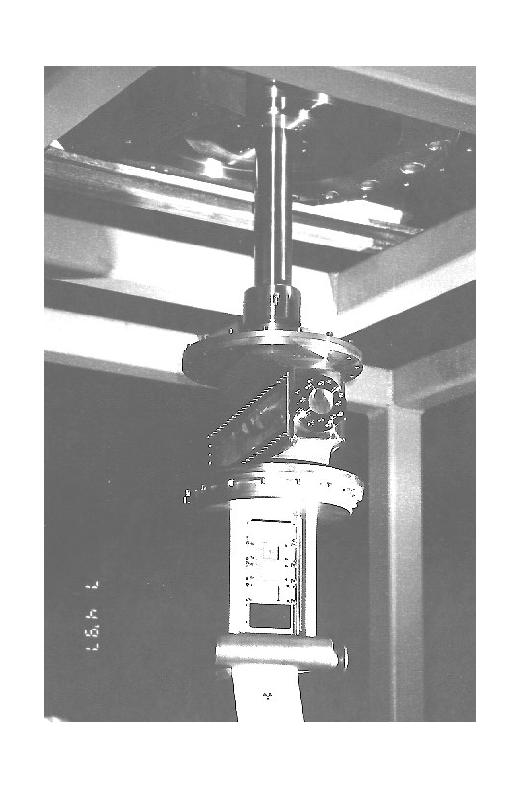
\includegraphics[  width=0.60\textwidth,
  height=0.60\textheight]{wt2_target_bw}\end{center}


\caption{Waterfall Target stack\label{fig: wt_target-stack}.}
\end{figure}



\section{Description of controls}

The software control of the target is written in EPICS and run on
the IOC \textit{iochawt1.} The IOC uses serial communication, DAC
and ADC to control the target. The pump motor tachometer, flowmeter,
position encoder, and home switch are read through the ADC card. It
is common to have noise on the flowmeter, tachometer, and encoder.
The user should expect this noise and not be alarmed. The user should
check the camara on the control rack to make sure that the postion
encoder does indicate the proper target (there is some acceptable
slop on this number).

The motion control is achieved via a SHS - APS 3/A stepper motor controller.
Communication with this controller is achieved through a RS232 serial
connection. This controller counts absolute steps from the home postion.
The home postion is defined using the HOME routine on the expert page
of the GUI. Non-Experts are forbidden to use this function as serious
down time may result. If the target motion mechanism does not seem
to be moving to the selected target, execution of the HOME routine
might be needed and an expert must be called.

The pump speed control is achieved through a -5 - 5V DAC. The DAC
is 12 bit and negative voltages are not used in the application. Therefore
the minimum set postion for the pump speed is 2048. This corresponds
to 0V and 0 pump speed (pump is off). A setting of 4095 corresponds
to 5 volts and maximum pump speed. It is not possible to set the pump
speed outside these limits in software.

A counter readout (ITECO trading mod. 9210001) provides the tachometer
signal. The signal output from the module is 4-20~mA which is converted
to 0-5V and connected to the ADC. There is significant noise on the
ADC channel which seems to be a feature of the ADC. The user should
expect this noise and not be alarmed at oscillating values for the
tachometer signal.

The same counter readout is used for the flowmeter. The device is
read using the same ADC and thus, the signal has a similar level of
noise. The user should expect this noise and not be alarmed at oscillating
values for the flowmeter signal.

The postion encoder is the same type used on the collimators for both
arms. The encoder is displayed using a simple digital display on the
control rack. This display unit has a 4-20~mA output that is converted
to 0-5V and connected to the ADC. Again, the ADC value has significant
noise. The user should expect this noise and not be alarmed at oscillating
values for the encoder signal.

Note that due to the oscillation of the signals from ADC, the user
operator should check the displays on the GUI with the displays visible
in the camara focused on the control rack.


\section{User operation}

The user GUI may by accessed from the Hall A main control screen using
the pull down menu. Figure \ref{fig: wt_GUI} shows the GUI. %
\begin{figure}
\begin{center}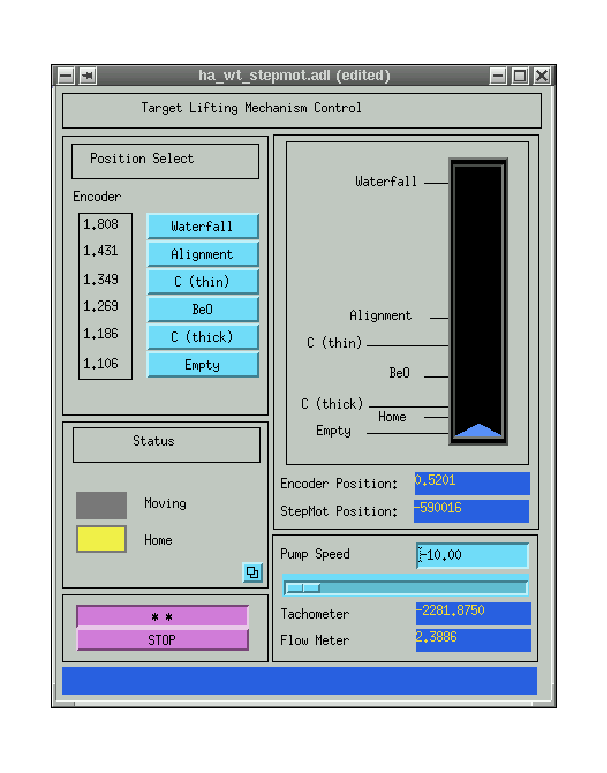
\includegraphics[  width=0.80\textwidth,
  height=0.60\textheight]{wt2_hawt-color}\end{center}


\caption{Target control GUI.\label{fig: wt_GUI}}
\end{figure}



\subsection{Target Selection}

The target postion is selected on the left side of the GUI under Position
Select. There are six options. The desired target is selected by clicking
on the particular target button. If the target is not already on the
desired postion, the user should see the {}``moving'' LED turn yellow
in the Status display. The graphic display to the right of the selection
boxes should update; the blue diamond indicating the current postion
of the target. In addition, the {}``Encoder Postion'' and {}``StepMot
Postion'' displays to the right of the GUI should update indicating
the target is in motion. If the motion does not appear to be operating
correctly, call an expert. At the end of the motion sequence the encoder
postion should be close to the value in text next to the target button.
The value on the camara should be within $\pm 0.0030$ on the encoder
readout. If this is not the case call an expert. Note that any target
motion will trip and FSD. The MCC should be informed of all target
motion. If for some reason during the target motion there is a need
to stop, click on the stop button. Motion can be restarted by selecting
another target.

There is an access from the {}``Status'' section to an expert screen.
Only experts should use the functions on this screen there are no
user features here.

In addition to the camara on the control rack, there is a camara on
top of the pivot focused on the motion mechanism. The target postions
and names are labled in a visible fashion. The user should double
check this camara as well to make sure the motion mechanism is behaving
as expected.

Finally, there are micro-switches that provide an FSD signal when
not on a target. If for some reason an FSD is still tripped after
a move to a new target, an expert should be called.


\subsection{Pump Speed Control}

The pump speed control is set using the slider bar or input field
in the {}``Pump Speed'' section. This input may range from 2048
to 4096 corresponding to a 12 bit DAC 0-5V output. The output of the
DAC is converted to 4-20 mA and used to control the pump speed. An
input of 2048 (0V) will stop the pump. An output of 4095 (5V) sets
the pump speed at $\sim 1800$ on the display which is roughly 6 l/min.
This should be more than adequate for normal operations. If the pump
does not function properly or more flow is desired, an expert must
be called. The tachometer and flowmeter displays should always be
checked with the displays on the camara.


\subsection{Rebooting the IOC}

The name of the IOC is iochawt1. The IOC may be rebooted by logging
into the IOC via telnet and typing reboot. If this is not possible,
(i.e. the IOC is not responding to remote login) call an expert.


\section{Troubleshooting (Experts only)}

This section is intended as a reference for experts only. Figure \ref{fig: wt_control rack}
shows the control rack. Figure \ref{fig: wt_IOC-rack} shows the IOC
rack.

%
\begin{figure}
\begin{center}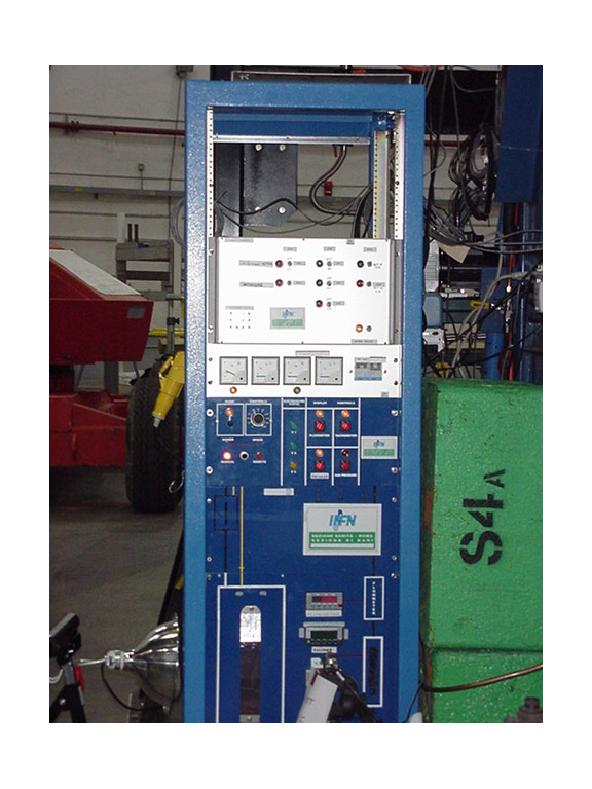
\includegraphics[  width=0.90\textwidth]{wt2_control-rack-color}\end{center}


\caption{Control rack for waterfall target.\label{fig: wt_control rack}}
\end{figure}
%
\begin{figure}
\begin{center}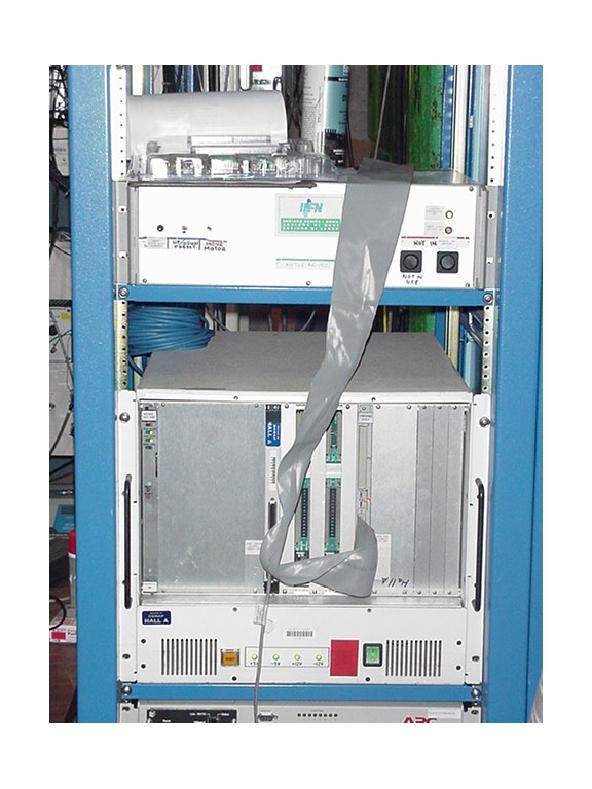
\includegraphics[  width=0.90\textwidth]{wt2_IOC-rack}\end{center}


\caption{IOC rack for waterfall target.\label{fig: wt_IOC-rack}}
\end{figure}



\subsection{Manual motion operation\label{sec: Manual}}

Ensure that the motor controller power is off. The power may be turned
off at the front of the main control rack under the beam line. In
the motor control rack located next to the IOC, there is a small chassis
mounted box. At the back of the box, there is a DIP switch clearly
marked with black pen labled B1. This switch must be set to OFF to
put the controller in manual mode. Restore power from the control
rack under the beam line. Return to the motor control box. If the
green LED at the right of the box turns on, all is well and the target
can be moved up or down by setting the direction switch and toggling
the move switch. To restore the remote operation of the system cut
power at the main control rack under the beam line. Return the B1
DIP switch to ON and restore power to the system. At this point the
controller does not {}``know'' where it is. The HOME routine must
now be run. See Section \ref{sec: HOME} for proper use of the HOME
routine.


\subsection{Use of the HOME routine\label{sec: HOME}}

Use of the HOME routine can be effected from them the main control
GUI. In the {}``Status'' section of the GUI, there is a small button
that brings up the expert page. Be sure that the physical position
of the target is a few centimeters above the H2O target. This can
be seen at the top of the scattering chamber. The HOME routine will
not properly execute from the H2O target postion. The target might
have to be moved manually above the H2O target postion (see Section
\ref{sec: Manual}). Press the HOME button. The target should move
in the direction of the HOME switch which is located near the empty
target position. If the target does not move in the correct direction,
move the target manually to some position close the the BeO target
position. This may take some time. The motor controller will look
for the HOME switch by moving the system up. When the HOME switch
is activated, the target will start moving down; when it finds the
HOME switch again it will stop. This ensures that the HOME position
is not affected by the hysteresis in the switch.


\subsection{Hardware limit over travel}

If a limit switch (either upper or lower) is tripped, the target motion
control system will lose power. This is designed so that the lifting
mechanism will not be damaged. In this case, the limit must be bypassed
and the target moved off of the limit manually. First, the controller
must be set to manual mode. See Section \ref{sec: Manual}. At the
front of the box, there is a switch labled bypass power. Turn this
switch down; the yellow LED above should turn on. Also on the front
of the box is limit switch bypass button. Press this button and move
the target manually. BE SURE TO MOVE IN THE CORRECT DIRECTION; severe
damage to the system may result from improper use of this feature.
If the motor does not seem to be moving, page Dave Meekins or Scot
Spiegel. As the power has been cycled to this module, it is now necessary
to run the home routine (see Section \ref{sec: HOME}). Disable bypass
power when finnished with motor reset.


\subsection{Manual water pump operation}

Operation of the water pump in the manual mode is simple. There is
a switch at the front of the main control rack (located under the
beam line) that can be toggled to remote or manual operation. The
pump power switch must be on for the pump to work. The pump speed
is controlled via the knob which can be rotated clockwise for more
speed. Please do not run the pump faster than 2000 as shown on the
tachometer display. This causes undue strain on the system.
% ===========  CVS info
% $Header: /group/halla/analysis/cvs/tex/osp/src/targets/waterfall-target.tex,v 1.2 2003/11/18 07:46:27 gen Exp $
% $Id: waterfall-target.tex,v 1.2 2003/11/18 07:46:27 gen Exp $
% $Author: gen $
% $Date: 2003/11/18 07:46:27 $
% $Name:  $
% $Locker:  $
% $Log: waterfall-target.tex,v $
% Revision 1.2  2003/11/18 07:46:27  gen
% waterfall docs collection
%
% Revision 1.1  2003/06/06 17:09:04  gen
% Revision printout changed
%
% Revision 1.2  2003/06/05 23:30:01  gen
% Revision ID is printed in TeX
%
% Revision 1.1.1.1  2003/06/05 17:28:27  gen
% Imported from /home/gen/tex/OSP
%
%  Revision parameters to appear on the output

